%-------------------------------------------------------------------------------
%	PACKAGES EN DOCUMENT CONFIGURATIE
%-------------------------------------------------------------------------------

\documentclass{uva-inf-article}
\usepackage[english]{babel}

\usepackage{tikz}
\usetikzlibrary{automata,positioning}

\usepackage{listings}

%-------------------------------------------------------------------------------
%	GEGEVENS VOOR IN DE TITEL
%-------------------------------------------------------------------------------

% Vul de naam van de opdracht in.
\assignment{Assignment 2}
% Vul het soort opdracht in.
\assignmenttype{Essay}
% Vul de titel van de eindopdracht in.
\title{Lexicographic Analysis}

% Vul de volledige namen van alle auteurs in.
\author{René Kok}
\uvanetid{13671146}

\author{Aram Mutlu}
\uvanetid{13574116}

% Vul eventueel ook de naam van de docent of vakcoordinator toe.
\docent{Dhr. dr. C.U. Grelck}
\course{Compiler Construction}
% Te vinden op onder andere Datanose.
\courseid{5062COMP6Y}

% Dit is de datum die op het document komt te staan. Standaard is dat vandaag.
\date{\today}

%-------------------------------------------------------------------------------
%	VOORPAGINA
%-------------------------------------------------------------------------------

\begin{document}
\maketitle

%-------------------------------------------------------------------------------
%	INHOUDSOPGAVE EN ABSTRACT
%-------------------------------------------------------------------------------

% Niet doen bij korte verslagen en rapporten
%\tableofcontents
%\begin{abstract}
%\lipsum[13]
%\end{abstract}

%-------------------------------------------------------------------------------
%	INTRODUCTIE
%-------------------------------------------------------------------------------

\section{Introduction}
\lipsum[1]

%-------------------------------------------------------------------------------
%	METHODE
%-------------------------------------------------------------------------------

\newpage
\section{Assignment}

\subsection{Thompson’s Construction}
\lipsum[1]
\begin{figure}[h]
    \centering
    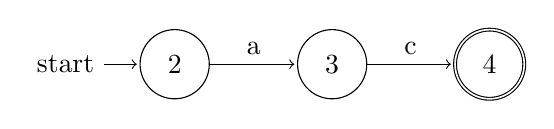
\begin{tikzpicture}[shorten >=1pt,node distance=2cm,on grid,auto] 
        \node[state, initial](2){2};
        \node[state, right=of 2](3){3};
        \node[state, accepting, right=of 3](4){4};
        \path[->] 
        (2) edge node {a} (3)
        (3) edge node {c} (4);
    \end{tikzpicture}
    \caption{Step 1 creating NFA for (ac) $\rightarrow$ (ac$\mid$ab)*}
    \end{figure}

    \begin{figure}[h]
        \centering
        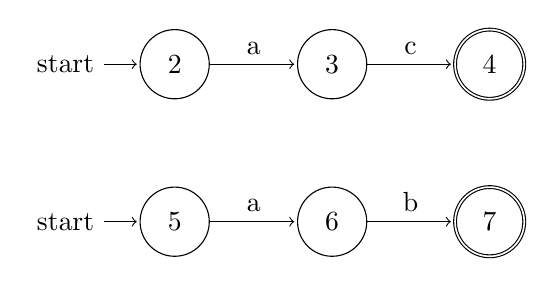
\begin{tikzpicture}[shorten >=1pt,node distance=2cm,on grid,auto]
            \node[state, initial](2){2};
            \node[state, right=of 2](3){3};
            \node[state, accepting, right=of 3](4){4};
            \node[state, initial, below=of 2](5){5};
            \node[state, right=of 5](6){6};
            \node[state, accepting, right=of 6](7){7};
            \path[->] 
            (2) edge node {a} (3)
            (3) edge node {c} (4) 
            (5) edge node {a} (6)
            (6) edge node {b} (7);
        \end{tikzpicture}
        \caption{Step 2 creating NFA for (ab) $\rightarrow$ (ac$\mid$ab)*}
        \end{figure}

        \begin{figure}[h]
            \centering
        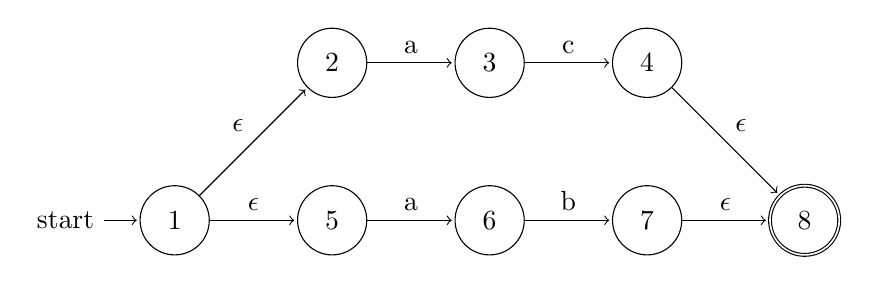
\begin{tikzpicture}[shorten >=1pt,node distance=2cm,on grid,auto] 
            \node[state, initial](1){1};
            \node[state, right=of 1](5){5};
            \node[state, above=of 5](2){2};
            \node[state, right=of 2](3){3};
            \node[state, right=of 3](4){4};
            \node[state, right=of 5](6){6};
            \node[state, right=of 6](7){7};
            \node[state, accepting, right=of 7](8){8};
            \path[->] 
            (1) edge node {$\epsilon$} (2)
                edge node {$\epsilon$} (5)
            (2) edge node {a} (3)
            (3) edge node {c} (4)
            (4) edge node {$\epsilon$} (8)
            (5) edge node {a} (6)
            (6) edge node {b} (7)
            (7) edge node {$\epsilon$} (8);
        \end{tikzpicture}
        \caption{Step 3 creating NFA for (ac|ab) $\rightarrow$ (ac$\mid$ab)*}
        \end{figure}        


\begin{figure}[h]
    \centering
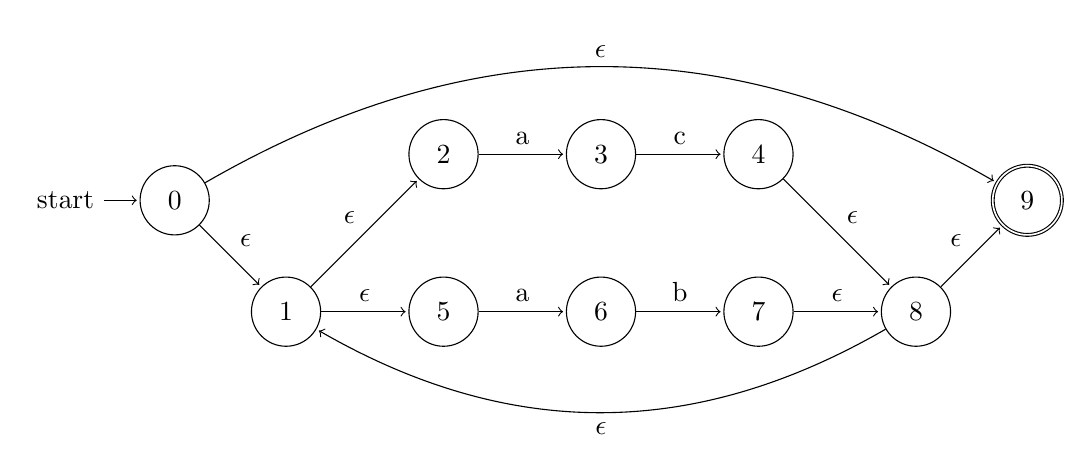
\begin{tikzpicture}[shorten >=1pt,node distance=2cm,on grid,auto] 
    \node[state, initial](0) {0};
    \node[state, below right=of 0](1){1};
    \node[state, right=of 1](5){5};
    \node[state, above=of 5](2){2};
    \node[state, right=of 2](3){3};
    \node[state, right=of 3](4){4};
    \node[state, right=of 5](6){6};
    \node[state, right=of 6](7){7};
    \node[state, right=of 7](8){8};
    \node[state, accepting, above right=of 8](9){9};
    \path[->] 
    (0) edge node {$\epsilon$} (1)
        edge [bend left] node {$\epsilon$} (9)
    (1) edge node {$\epsilon$} (2)
        edge node {$\epsilon$} (5)
    (2) edge node {a} (3)
    (3) edge node {c} (4)
    (4) edge node {$\epsilon$} (8)
    (5) edge node {a} (6)
    (6) edge node {b} (7)
    (7) edge node {$\epsilon$} (8)
    (8) edge node {$\epsilon$} (9)
        edge [bend left] node {$\epsilon$} (1);
\end{tikzpicture}
\caption{Final non-deterministic finite automaton for "(ac$\mid$ab)*"}
\end{figure}
\subsection{Subset Construction}
\lipsum[1]
\subsection{Hopcroft’s Algorithm}
\lipsum[1]
\subsection{Direct-coded Scanner}
\lipsum[1]
\lstinputlisting[language=C]{code.c}
\end{document}